\section{Path-View}\label{sec:pathgate}
\textbf{Notation:} We consider fully connected deep networks with $d$ layers, and $w$ hidden units per layer, which accepts an input $x\in\R^{d_{in}}$, and produces an output $\hat{y}_{t}\in \R$. We denote by $\Theta(l,i,j)$ to be the weight connecting the $i^{th}$ hidden unit of layer $l-1$ to the $j^{th}$ hidden unit of layer $l$, and we use $G_{x,t}(l,i)$ be the gating value ($0/1$) of the $i^{th}$ hidden unit in layer $l$ for an input $x\in \R^{d_{in}}$.\\
\textbf{Paths:}  We have a total of $P=d_{in}w^{(d-1)}$ paths. Let us say that an enumeration of the paths is given by $[P]=\{1,\ldots,P\}$. Let $\I_{l}\colon [P]\ra [w],l=0,\ldots,d-1$ provide the index of the hidden unit through which a path $p$ passes in layer $l$ (with the convention that $\I_d(p)=1,\forall p\in [P]$). The activity of a path $p$ for an input $x\in \R^{d_{in}}$ by $A_{t}(x,p)\stackrel{def}{=}\Pi_{l=1}^{d-1} G_{x,t}(l,\I_l(p))$.\\
\textbf{Neural Path Feature (NPF)} of an input example $x\in \R^{d_{in}}$ is given by \begin{align}\label{eq:npf}\phi_{x,t}=(x_s(\I_0(p))A_t(x_s,p) ,p\in[P])\in\R^P,\end{align} where, for a path $p$, $\I_0(p)$ is the input node at which the path starts, and $A_t(x_s,p)$ is its activity. %By arranging the NPF of the $n$ input examples in a matrix $\Phi_t=(\phi_{x_s,\G_t},s\in[n])\in\R^{P\times n}$, we can express 
\textbf{Neural Path Value (NPF)} is given by \begin{align}\label{eq:nfv}v_{t}=(\Pi_{l=1}^d \Theta_t(l,\I_{l-1}(p),\I_l(p)),p\in[P])\in\R^P\end{align}
The zeroth and first-order terms of a DNN can be written as:
\begin{align}
\label{eq:zero}\text{(Zeroth-Order)}\quad: \quad \hat{y}_t(x)&=\ip{\phi_{x,t},v_t}=\sum_{p\in [P]}x(\I(p))A_t(x,p)v_t(p)\\
\label{eq:first}\text{(First-Order)}\quad: \quad \partial \hat{y}_t(x)&=\underbrace{\ip{\phi_{x,t},\partial v_t}}_{\text{value gradient}}+ \underbrace{\ip{\partial\phi_{x,t},v_t}}_{\text{feature gradient}}\\&=\sum_{p\in [P]}x(\I(p)) A_t(x,p) \partial(v_t(p))+\sum_{p\in [P]}x(\I(p)) \partial(A_t(x,p)) v_t(p)\nn
\end{align}
\subsection{Information Flow: Zeroth-Order}
$1.$ \textbf{Representational Power:} The ability of DNNs to fit data has been demonstrated in the past. \cite{ben} showed that DNNs can fit even random labels, and random pixels of standard datasets such as MNIST. However, we note that, for standard DNNs with ReLU gates, with no bias parameters, a dataset with $n=2$ points namely $(x,1)$ and $(2x,-1)$ for some $x\in \R^{d_{in}}$ cannot be memorised. The reason is that the gating values are the same for both $x$ and $2x$ (for that matter any positive scaling of $x$), and hence $\phi_{2x,\G_t }= 2\phi_{x,\G_t }$, and thus it not possible to fit arbitrary values for $\hat{y}_t(x)$ and $\hat{y}_t(2x)$.\\
$2.$ \textbf{Translation Invariance:} Consider a convolution network using $l$ layers of circular convolutions\footnote{Here, instead of zero-padding in the corners, we follow the convention that index $d_{in}+k$ will be interpreted as $k$, for $k>0$, and $-k$ will be interpreted as $d_{in}-k$.} with filter size $k'<d_{in}$ and unit stride, and let $x^l(i)$ be the output of the $i^{th}$ channel after either $\max$-/global-average-pooling. Looking at the third and fourth (from left) illustrations in \Cref{fig:cartoon}, it is easy to check the translation invariance property: each of the red, blue, green lines have the same path values due to weight sharing in the convolutional layers, this leads to a circular symmetry in the path values, due to which, a translation in the input will cause all the internal variable to translate, and final invariance results from the invariance of the $\max$/average operation.\\
$3.$ \textbf{Active Sub-Network:} At any time $t$, for each input example, a set of gates are \emph{on} in each layer, and this gives rise to the sub-network of active paths for that input. Thus the active sub-network can be said to hold the memory for a given input. It easy to check that the \emph{neural path kernel} NPK associated with the NPF satisfies the property $H_t=\Sigma\odot \lambda_t$, where $\Sigma$ is the $n\times n$ input Gram matrix, $\odot$ is the \emph{Hadamard} product, and $\lambda_t(s,s')\stackrel{def}{=}\sum_{p\rsa i} A_t(x_s,p) A_t(x_{s'},p)$ is the overlap of the sub-networks that are active for both input examples $s,s'\in[n]$.
\begin{figure*}[t]
%\begin{minipage}{0.78\columnwidth}
\resizebox{\columnwidth}{!}{
\begin{tabular}{ccc}
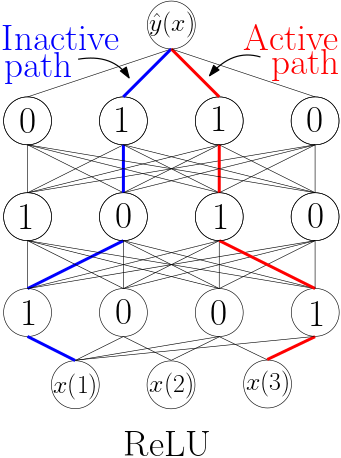
\includegraphics[scale=0.5]{figs/nn.png}
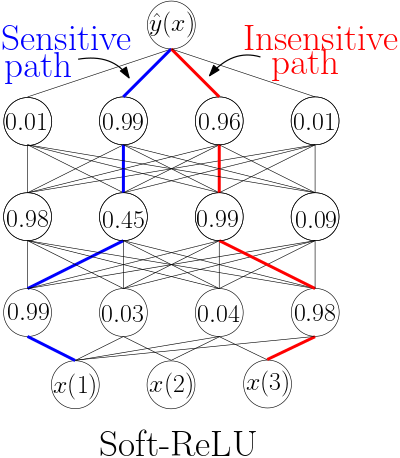
\includegraphics[scale=0.5]{figs/nnsoft.png}
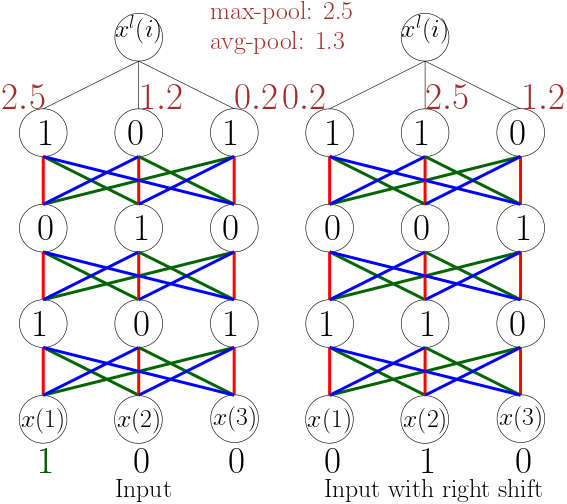
\includegraphics[scale=0.5]{figs/nnconv.png}
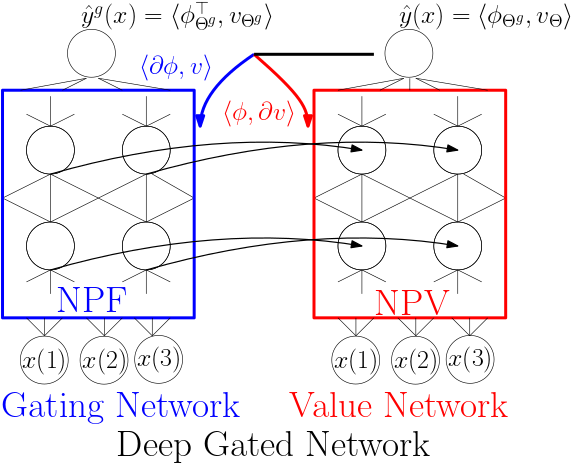
\includegraphics[scale=0.5]{figs/nntwin-blck.png}
%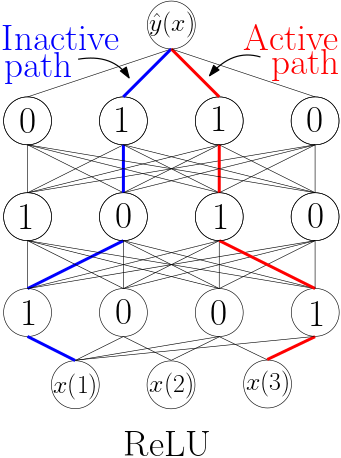
\includegraphics[scale=0.5]{figs/nn.png}
%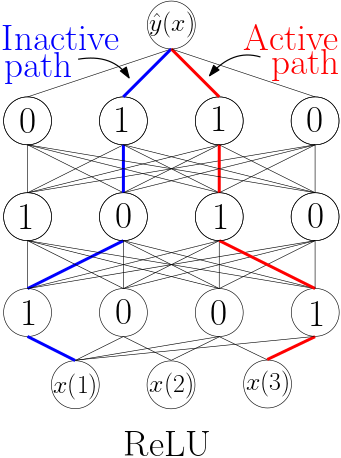
\includegraphics[scale=0.5]{figs/nn.png}
\end{tabular}
}
%\end{minipage}
%\begin{minipage}{0.18\columnwidth}
%\resizebox{\columnwidth}{!}{
%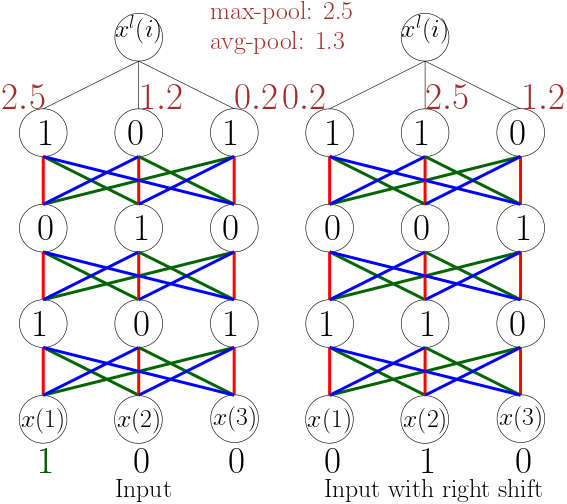
\includegraphics[scale=0.5]{figs/nnconv.png}
%}
%\end{minipage}
\caption{Cartoon illustration of usefulness of path-view and DGN framework.}
\label{fig:cartoon}
\end{figure*}
\subsection{Information Flow: First-Order}
$1.$ \textbf{Value Gradient} $\ip{\phi_{x,t},\partial v_t}$ (see \eqref{eq:zero}) flows through the active sub-network. To see this, $\ip{\phi_{x,t},\partial v_t}=\sum_{p\in[P]}x(\I_0(p))A(x,p)\partial v$, i.e., only paths $p$ with $A(x,p)=1$ contribute to the summation and the derivate $\partial v(p)$ is non-zero only for those weights through which the path $p$ passes.\\
$2.$ \textbf{Feature Gradient and fixing the ReLU artefact:} The \emph{feature derivative} given by $\ip{\partial\phi_{x,t},v_t}=\sum_{p\in [P]}x(\I(p)) \partial(A_t(x,p)) v_t(p)$. Note that, in the case of ReLU activations the gating values are either $0$ or $1$, and hence $\partial(A_t(x,p))=0$. However, the gating values and hence the path activities $A_t(\cdot,\cdot)$ changes during training. This artefact arising due to non-differentiability can be fixed by considering a \emph{soft-ReLU} activation, where, for a pre-activation input $q\in\R$ the output is given by $q\frac{1}{1+\exp(-\beta q)}$ as opposed to $q\mathbbm{1}_{\{q>0\}}$ of the ReLU. Soft-ReLU enables us to capture the terms related to feature learning in our analysis. The difference between hard and soft gates can be seen in the first two illustrations in \Cref{fig:cartoon}, where negative/positive values lead to $0/1$ in the case of hard gating, and close to $0/1$ in the case of soft-gating.\\
$3.$ \textbf{Sensitive Sub-Network:} At any time $t$, for each input example, the set of paths for which $\partial A(x,p)$ is significant, form the sensitive sub-network for that input. It is easy to check in a DNN with soft-ReLU, that an active path $p$ whose gating values are close to $1$ is not sensitive, because, $\partial A(x,p)$ will be close to $0$. Thus, the active sub-network and sensitive sub-network are non-overlapping, as shown in the first two illustrations of \Cref{fig:cartoon}, where the red active path is insensitive and the blue inactive path is sensitive. The active paths are responsible for holding the memory of a given input and the sensitive paths are the ones which contains gates whose gating values can go towards $1/0$ depending on flow of feature gradient. In the case, of ReLU gates, sensitive paths are those which involve gates whose pre-activation inputs are close to $0$, and are in the verge of either turning \emph{on/off} depending on gradient flow.
\subsection{Deep Gated Network (DGN)}
The NPFs are zeroth-order features stored solely in the gates of a DNN. In this paper, we separate out the NPFs from the NPVs. To this end, we introduce the deep gated network (DGN) framework, wherein, the output of a hidden unit is obtained as a product of its pre-activation and a gating value. A DGN has two network namely i) the gating network which holds the gating values and hence the NPF, and ii) a value network which holds the NPVs. %We denote a DNG by $\N(\Theta_t;\G(\Tg_t,\beta)$ or simply $\N(\Theta_t;\Tg_t,\beta)$
\FloatBarrier
\begin{table}[h]
\begin{minipage}{0.5\columnwidth}
\resizebox{\columnwidth}{!}{
\begin{tabular}{|c|c|}\hline
Gating Network: $\G(\Tg_t,\beta)$\\\hline
$z_{x,\Tg_t}(0)=x$  \\\hline
$q_{x,\Tg_t}(l)={\Tg_t(l)}^\top z_{x,\Tg_t}(l-1)$ \\\hline
$z_{x,\Tg_t}(l)=q_{x,\Tg_t}(l)\odot G_{x,\Tg_t}(l)$ \\\hline
{$\begin{aligned}\beta >0: G_{x,\Tg_t}(l,i)&=\frac{1+\epsilon}{1+\exp(-\beta q_{x,\Tg_t}(l,i))} \\ \beta=\infty: G_{x,\Tg_t}(l,i)&=\mathbbm{1}_{\{q_{x,\Tg_t}(l,i)>0\}}\end{aligned}$}\\\hline 
\end{tabular}
}
\end{minipage}
\begin{minipage}{0.5\columnwidth}
\resizebox{\columnwidth}{!}{
\begin{tabular}{|l|l|}\hline
\multicolumn{2}{|c|}{Value Network: $\N(\Theta_t;\G_t)$}\\\hline 
Input layer & $z_{x,\Theta_t}(0)=x$ \\\hline
Pre-activation & $q_{x,\Theta_t}(l)={\Theta_t(l)}^\top z_{x,\Theta_t}(l-1)$\\\hline
Layer output & $z_{x,\Theta_t}(l)=q_{x,\Theta_t}(l)\odot G_{x,t}(l)$ \\\hline
Final output & $\hat{y}_t(x)={\Theta_t(d)}^\top z_{x,\Theta_t}(d-1)$\\\hline
Gating Values& $\begin{aligned}\G_t\stackrel{def}=\{G_{x_{s},t}(l,i), \forall s\in[n],\\l\in[d-1],i\in[w]\}\end{aligned}$\\\hline
\end{tabular}
}
\end{minipage}
\caption{$q(l),z(l)$ and $G(l)$ are $w$-dimensional quantities. At time $t$, by specifying the gating values for all the $n$ input examples as $\G_t\stackrel{def}=\{G_{x_{s},t}(l,i), \forall s\in[n],l\in[d-1],i\in[w]\}$, we can recover the outputs $\hat{y}_t(x_s)\in \R$ for all the inputs $\{x_s\}_{s=1}^n$ in the dataset.}
\label{tb:dgn}
\end{table}
